The \emph{ed\_localization}\footnote{\url{https://github.com/tue-robotics/ed_localization}} plugin implements \acrshort{amcl} based on a 2D render of the central world model.With use of the \emph{ed\_navigation} plugin\footnote{\url{https://github.com/tue-robotics/ed_navigation}}, an occupancy grid is derived from the world model and published. With the use of the \emph{cb\_base\_navigation} package\footnote{\url{https://github.com/tue-robotics/cb_base_navigation}} the robots are able to deal with end goal constraints. The \emph{ed\_navigation} plugin allows to construct such a constraint w.r.t. a world model entity in \acrshort{ed}. This enables the robot to navigate not only to areas or entities in the scene, but to waypoints as well. Figure \ref{fig:ed_segmentation} also shows the navigation to an area.
% as illustrated by Figure \ref{fig:ed_navigation_constraints}.
Modified versions of the local and global ROS planners available within \emph{move\_base} are used.
\begin{figure}[H]
	\centering
	%\vspace{-0.3cm}
	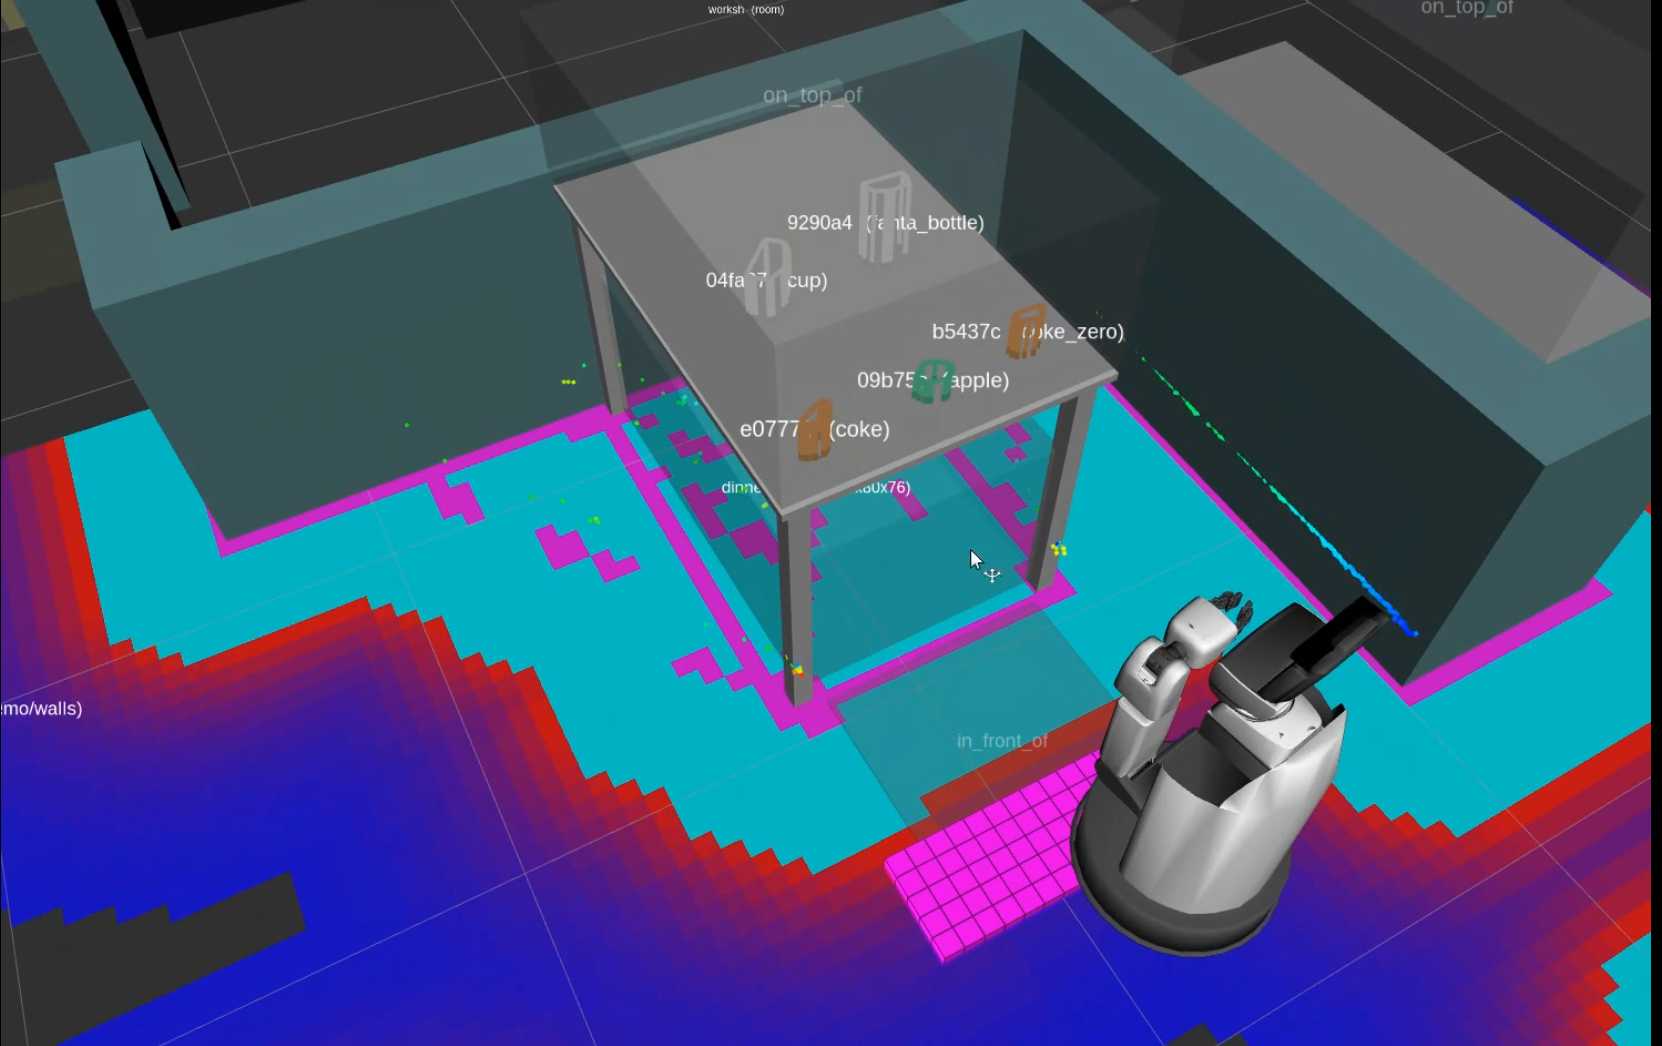
\includegraphics[width = 0.8\linewidth]{Figures/ed_segmentation_hsr}
	%\vspace{-0.5em}
	\caption{A view of the world model created with \acrshort{ed}. The figure shows the occupancy grid as well as classified objects recognized on top of the cabinet.}
	\label{fig:ed_segmentation}
	%\vspace{-0.5cm}
\end{figure}
